


\usebackgroundtemplate{
	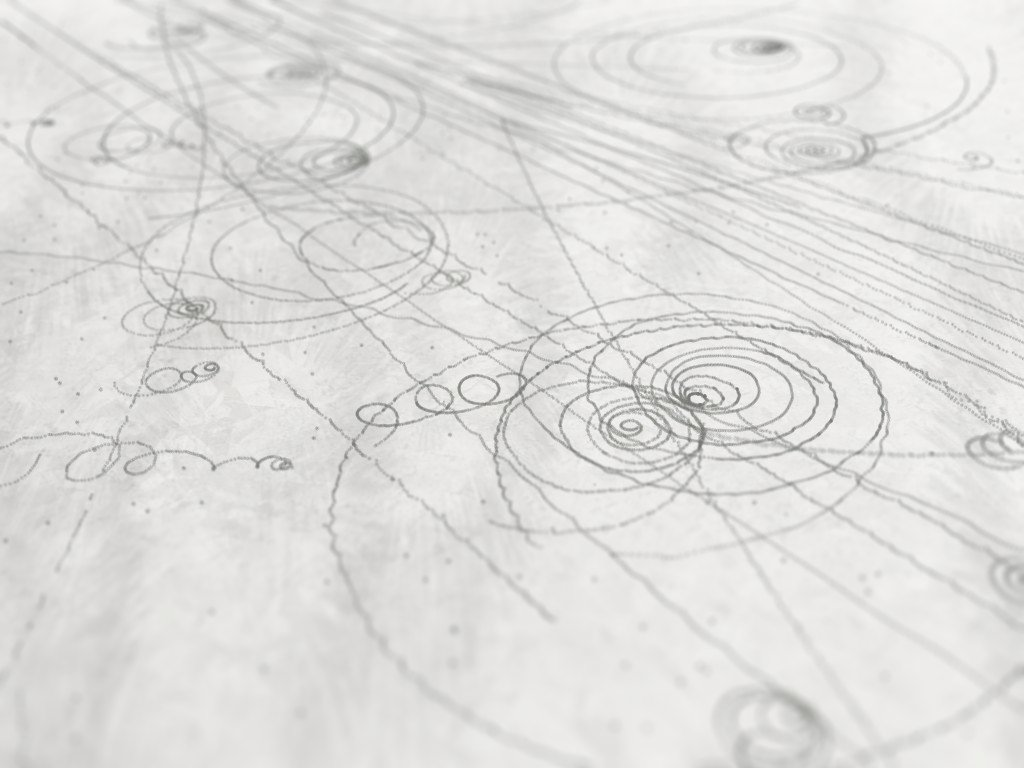
\includegraphics[width=\paperwidth,height=\paperheight]{logos/Blasenkammer_by_HenryGale_white}%
}






%% ------------------------------------------------------------
%% ------------------------------------------------------------
\subsection{Table}
%% ------------------------------------------------------------
%% ------------------------------------------------------------
\color{titlecolor}
\usebackgroundtemplate{
	\includegraphics[width=\paperwidth,height=\paperheight]{}%
}
\begin{frame}
 % \frametitle{\dataSample}
  \frametitle{ECAL scale}
  \framesubtitle{\invMassVarName }
  %RERECOTAG
  %PERIOD
\\
  Fit with convoluted Breit-Wigner (BW) and Crystal Ball (CB).

  %  \bl
  %   $\Delta m$: shift of the peak position of the CB

  \dualslide{
    $$ \Delta P = \frac{\Delta m_{data} - \Delta m_{MC}}{m_{Z}}$$
  }{  
    \begin{description}
    \item [golden:] $R9 > 0.94$
    \item [showering:] $R9 < 0.94$
    \end{description}
  }
  
  \begin{center}
    \emph{\dataSample}\xspace \invMassVarName

    \begin{tabular}{|l|c|*{3}{c|}} \hline
      ECAL Region of & selected  & $\Delta m_{data}$ & $\Delta m_{MC}$  & $\Delta$P (\%) \\
      the two electrons & events & (GeV) & (GeV) & \\
      \hline
      \hline
      _TABLE_
      \hline		
    \end{tabular}
  \end{center}


\end{frame}


\begin{comment}
%% ------------------------------------------------------------
\color{titlecolor}
\begin{frame}
  \frametitle{Fit Method: Old Additional smearing}
  \framesubtitle{\invMassVarName}
\\
  Fit with convoluted Breit-Wigner (BW) and Crystal Ball (CB).

  %  \bl
  %   $\Delta m$: shift of the peak position of the CB

  \dualslide{
    %      $$ \Delta P = \frac{\Delta m_{data} - \Delta m_{MC}}{m_{Z}}$$
    $$ \Delta \sigma = \frac{\sqrt{2}}{M_Z} \sqrt{(\sigma_{CB}^{data})^2 - (\sigma_{CB}^{MC})^2}$$    
  }{  
    \begin{description}
    \item [golden:] $R9 > 0.94$
    \item [showering:] $R9 < 0.94$
    \end{description}
  }
  
  \begin{center}
    \emph{\dataSample}\xspace \invMassVarName

    \begin{tabular}{|l|c|*{3}{c|}} \hline
      ECAL Region of & selected  & $\sigma_{CB}^{data}$ & $\sigma_{CB}^{MC}$  & $\Delta \sigma$ (\%) \\
      the two electrons & events & (GeV) & (GeV) & \\
      \hline
      \hline
      _TABLESIGMA_
      \hline		
    \end{tabular}
  \end{center}
\end{frame}
\end{comment}


%% ------------------------------------------------------------

%% ------------------------------------------------------------
\color{titlecolor}
\begin{frame}
 % \frametitle{\dataSample}
  \frametitle{Fit Method: New Additional smearing}
  \framesubtitle{\invMassVarName}
 \\
  Fit with convoluted Breit-Wigner (BW) and Crystal Ball (CB).

  %  \bl
  %   $\Delta m$: shift of the peak position of the CB
  $$ \text{add. smear.}  = \sqrt{2 \cdot \left( \left(\resol^{data}\right)^2 - \left(\resol^{MC}\right)^2 \right)}$$

  %%     \dualslide{
  %% %      $$ \Delta P = \frac{\Delta m_{data} - \Delta m_{MC}}{m_{Z}}$$
  %% %      $$ \Delta \sigma = \frac{\sqrt{2}}{M_Z} \sqrt{(\sigma_{CB}^{data})^2 - (\sigma_{CB}^{MC})^2}$$    
  %%       add. smear. $ = \sqrt{(2 \cdot (\resol^{data})^2 - (\resol^{MC})^2$ 
  %%     }{  
  %%       \begin{description}
  %%       \item [golden:] $R9 > 0.94$
  %%       \item [showering:] $R9 < 0.94$
  %%       \end{description}
  %%     }
  
  \begin{center}
    \emph{\dataSample}\xspace \invMassVarName

    \begin{tabular}{|l|c|c|c|c|} \hline
      ECAL Region of & selected  & $\resol^{data}$ & $\resol^{MC}$  & add. smear. \\
      the two electrons & events & (\%) & (\%) & (\%) \\
      \hline
      \hline
      _TABLESIGMANEW_
      \hline		
    \end{tabular}
  \end{center}
\end{frame}


%% ------------------------------------------------------------
